\section{Introduction}

Locating visual landmarks, such as human body joints \cite{toshev2014deeppose} and facial key points \cite{xiong2013supervised}, is an important yet challenging problem. The stacked U-Nets, {\it e.g.} hourglasses (HGs) \cite{newell2016stacked}, are widely used in landmark localization. Generally speaking, their success can be attributed to design patterns: 1) within each U-Net, connect the top-down and bottom-up feature blocks to encourage gradient flow; and 2) stack multiple U-Nets in a cascade to refine prediction stage by stage.

However, the shortcut connection exists only ``locally'' inside each U-Net \cite{ronneberger2015u}. There is no ``global'' connection across U-Nets except the cascade. Blocks in different U-Nets cannot share features, which may impede the information flow and lead to redundant parameters.

We propose densely connected U-Nets (DU-Net) to address this issue. The key idea is to directly connect blocks of the same semantic meanings, {\it i.e.} having the same resolution in either top-down or bottom-up context, from any U-Net to all subsequent U-Nets. Please refer to Fig. \ref{fig:framework} for an illustration. The dense connectivity is similar to DenseNet \cite{huang2016densely} but generalizing the design philosophy from feature to semantic level. It encourages information flow as well as feature reuse ``globally'' across the stacked U-Nets, yielding improved localization accuracy. 

Yet there are critical issues in designing DU-Net: 1) The number of parameters would have a quadratic growth since $n$ stacked U-Nets could generate $O(n^2)$ connections. 2) A naive implementation may allocate new memory for every connection, making the training highly expensive and limiting the maximum depth of DU-Nets. 

% The training would be extremely memory expensive since a naive implementation has to make a copy of every connected feature for network forward and back propagation.  



\begin{figure*}[t!]
\centering
  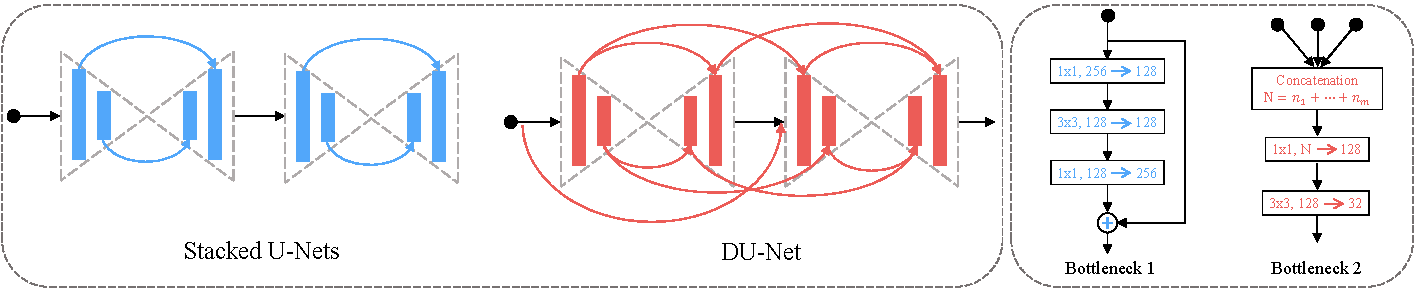
\includegraphics[width=1.0\linewidth]{figures/framework-cropped.pdf}
\caption{Illustration of stacked U-Nets and DU-Net. Stacked U-Nets has skip connections only within each U-Net. In contrast, DU-Net also connects blocks with the same semantic meanings across different U-Nets. The feature reuse could significantly reduce the size of bottleneck in each block, as shown in the right figure. Consequently, with the same number of U-Nets, DU-Net has only 30\% parameters of stacked U-Nets.}
\label{fig:framework}
\end{figure*}

% 
Our solution to those efficiency issues is threefold. {\bf First}, instead of connecting all stacked U-Nets, we only connect a U-Net to its $K$ successors. We name it as the $order$-$K$ connectivity, which aims to balance the fitting accuracy and parameter efficiency by cutting off long-distance connections. {\bf Second}, we employ a memory-efficient implementation in training. The key idea is to reuse a pre-allocated memory so all connected blocks could share the same memory. Compared with the naive implementation, this strategy makes it possible to train a very deep DU-Net (actually, $2\times$ deeper). {\bf Third}, to further improve the efficiency, we investigate an iterative design that may reduce the model size to one half. More specifically, the output of the first pass of the DU-Net is used as the input of the second pass, where detection or regression loss is applied as supervision. 

% %G%
% In view of deploying our approach on mobile devices, we further attempt to quantize weights, inputs, and gradients of DU-Net to low bit-width discrete values. This not only decreases the high precision operations but also shrinks the memory usage during training. By network quantization, the size of trained model can also be largely compressed.
% %G%
Besides shrinking the number of network parameters, we also study to further quantize each parameter. This motivates from the ubiquitous mobile applications. Although current mobile devices could carry models of dozens of MBs, deploying such networks requires high-end GPUs. However, quantized models could be accelerated by some specifically designed low-cost hardwares. Beyond only deploying models on mobile devices \cite{li2017deeprebirth}, training deep neural networks on distributed mobile devices emerges recently \cite{mcmahan2016communication}. To this end, we also try to quantize not only the model parameters but also its inputs (intermediate features) and gradients in training. This is the first attempt to investigate training landmark localizers using quantized inputs and gradients.


In summary, our key contributions are:
\begin{itemize}
    \item To the best of our knowledge, we are the first to propose quantized densely connected U-Nets for visual landmark localization, which largely improves the information flow and feature reuse at the semantic level.
    \item We propose the $order$-$K$ connectivity to balance accuracy and efficiency. It decreases the growth of model size from quadratic to linear by removing trivial connections. Experiments show it could reduce $\sim$70\% parameters of state-of-the-art landmark localizers.
    \item Very deep U-Nets can be trained using a memory-efficient implementation, where pre-allocated memory is reused by all connected blocks.
    \item We further investigate an iterative refinement that may cut down half of the model size, by forwarding DU-Net twice using either detection or regression supervision.
    %G%
    \item Different from previous efforts of quantizing only the model parameters, we are the first to quantize their inputs and gradients for better training efficiency on landmark localization tasks. By choosing appropriate quantization bit-widths for weights, inputs and gradients, quantized DU-Net achieves $\sim$75\% training memory saving with comparable performance. 
    %G%
    \item Exhaustive experiments are performed to validate DU-Net in different aspects. In both human pose estimation and face alignment, DU-Net demonstrates comparable localization accuracy and use $\sim$2\% model size compared with state-of-the-art methods.
\end{itemize}

% We are the first to deploy network quantization for better training efficiency on localization tasks. By choosing appropriate quantization bit-widths for weights, inputs and gradients, quantized DU-Net achieves at least 32$\times$ memory saving with comparable performance to the-state-of-art approaches. 


%The landmark localization such as human pose estimation \cite{toshev2014deeppose,newell2016stacked,wei2016convolutional}, facial landmark localization \cite{xiong2013supervised,zhang2014facial,sagonas2013300}, etc, plays an important role in the higher-level image understanding. The Convolutional Neural Networks (CNNs) have dominated this field, among which recent architecture of stacked hourglasses \cite{newell2016stacked}, a variant of the U-Net \cite{ronneberger2015unet}, becomes a standard solution. The skip connections between top-down and bottom-up blocks within a U-Net could preserve the spatial information and increase the gradient flow. With multiple U-Nets stacked together, the prediction could be refined stage by stage. However, the connections are only within each U-Net of the stacked hourglasses and no explicit connections exist between U-Nets, which may impede the information flow across them. And the blocks with the same semantics in different U-Nets cannot share features, leading to many redundant parameters. 

% Its success attributes to three key factors: repeated top-down, bottom-up inferences, intermediate supervisions and residual bottlenecks \cite{}. 

% The multiple stage top-down and bottom-up processing could better integrate both the local and global visual contexts into the final prediction. The intermediate supervision and residual bottlenecks, on the other hand, could alleviate the gradient vanish problem in deep networks.
%In this paper, we propose to densely connect stacked U-Nets by linking blocks with the same semantics in different U-Nets. We refer to this architecture as {\it Dense U-Nets}. The blocks in a U-Net could get direct inputs from its connected blocks in all preceding U-Nets, making the information flow more efficiently among the U-Nets. The feature reuse at each resolution could reduce the parameters in each block. The dense connectivity in our Dense U-Nets is different from that of DenseNet \cite{huang2016densely}. More specifically, layers only within each single block of the DenseNet are connected. In contrast, we connect blocks lying across the whole Dense U-Nets and connections of hierarchical blocks are mixed together. An illustration is given in Figure \ref{fig:framework}. We name it as the {\it global dense connectivity} to differentiate from the local one in the DenseNet.

% Besides, features in the Dense U-Nets are fused by the concatenation which could facilitate the information flow compared with the summation operation in the stacked hourglasses.

% Although the dense connectivity in our Dense U-Nets is similar with that of DenseNet \cite{}, 
% More recently, the DenseNet \cite{} achieves superior image classification performance over the ResNet \cite{} in terms of both the accuracy and model size, which benefits from the dense connections between layers. Its key insight is the feature reuse between layers of the same resolutions. The dense connectivity in the DenseNet, existing within one block, is local. By extending this principle, we propose a global dense connectivity, in contrast to the local connectivity in \cite{}, that blocks at the same locations of different U-Nets are connected. Hence, we refer to this architecture as {\it Dense U-Nets}. To our best knowledge, we are the first to generalize the local dense connectivity into the stacked U-Nets. 
% The global dense connectivity could make it easier to train much deeper stacked U-Nets.

% This motivates us to replace the residual modules  in the stacked hourglasses with the dense connected layers. However, this dense connectivity exists only locally within a contiguous  block in which all feature maps have the same spatial resolution. A U-Net, on the other hand, consists of a sequence of top-down and bottom-up blocks. A straight way is to turn each block into a dense block with multiple layers. However, this would sacrifice the spirit of stacked hourglasses that multiple stacked hourglasses outperform a single hourglass with multiple layers in each block.

% In order to integrate the structure of stacked U-Nets together with the idea of dense connectivity, we propose a global dense connectivity, in contrast to the local connectivity in \cite{}, that blocks at the same locations of different U-Nets are connected. Hence, we refer to this architecture as {\it Dense U-Nets}. The connected layers in the Dense U-Nets distribute along the whole network rather than in local continuous blocks. Compared with the local residual modules in the stacked hourglasses, the global dense connections could significantly facilitate the gradient to flow across stacked U-Nets.

%In practice, the Dense U-Nets have the efficiency problems of both parameter and training memory. First, suppose a Dense U-Nets contains $n$ U-Nets, there would be $O(n(n-1)/2)$ connections. Even though we use the dense bottleneck in Figure \ref{fig:framework}, the number of conv($1\times 1$) parameters still has the quadratic growth. Inspired from the Variable Order Markov (VOM) models \cite{begleiter2004prediction}, we propose the order-K connectivity that, instead of linking all the U-Nets, we connect only a fixed number of U-Nets. The goal is to use the minimum connections achieving the most obvious improvements. The multiple intermediate supervisions in the Dense U-Nets are good compensates for the order-K connectivity since they could provide additional gradients. The DenseNet does not have this advantage since it has only one supervision at the end.

% Furthermore, different from the DenseNet with only one supervision, the Dense U-Nets have multiple intermediate supervisions. The global dense connections plus the intermediate supervisions could bring faster convergence on the training set, but also gives rise to the concern of overfitting. Inspired from the Variable Order Markov (VOM) models \cite{}, we propose the order-K connectivity that, instead of linking all the U-Nets, we connect only a fixed number of U-Nets. The goal is to use the minimum connections achieving the most obvious improvement. Another advantage of order-K connectivity is that it has fewer parameters compared with the dense connectivity.

%Benefiting from the order-K connectivity, the Dense U-Nets could achieve comparable performance of stacked hourglasses with only one-third parameters. However, a naive implementation of the order-K connectivity could make the training very memory expensive. Therefore, we employ the memory efficient implementation \cite{pleiss2017memory}. The key idea is to share memories for time efficient operations such as concatenation and batch norm \cite{ioffe2015batch} within the connected layers. By pre-allocating a fixed memory, the later features produced by these operations would replace earlier features. So we need to re-compute those replaced features in the backward phase. The memory efficient implementation makes it possible to train Dense U-Nets two times deeper than the stacked hourglasses. 

%Furthermore, we also investigate to use the iterative refinement improving the parameter efficiency. Given a Dense U-Nets, we compare its performance with another Dense U-Nets with only half depth but an additional iteration. Besides, both detection and regression losses \cite{bulat2016human} were used in the landmark detection tasks, but there is no investigation yet about how they independently and collaboratively affect the prediction. We will give their detailed comparison in our experiments.

%In summary, the key contributions are:
%\begin{itemize}
%    \item To our best knowledge, we are the first to use the dense connectivity among the stacked U-Nets. The global dense connectivity in our Dense U-Nets is different from the local one in the DenseNet \cite{huang2016densely}.
%    \item We propose the order-K connectivity to make the Dense U-Nets parameter efficient. The order-K connectivity could decrease the growth of conv($1\times 1$) parameters from quadratic to linear. With comparable performance as the stacked hourglasses \cite{newell2016stacked}, it makes the Dense U-Nets require only one-third parameters. 
%    \item The memory efficient implementation of Dense U-Nets is provided to reduce its training memory usage. It makes it possible to train Dense U-Nets two times deeper than the stacked hourglasses.
%    \item We further explore using iterative refinement to improvement the parameter efficiency. At the same time, we investigate how different combinations of the detection and regression losses affect the performance.
%\end{itemize}